\section{Results and Discussion}

% Wide figures are declared before the running text so the compositor can fill each page.

\begin{figure*}[!tbp]
\centering
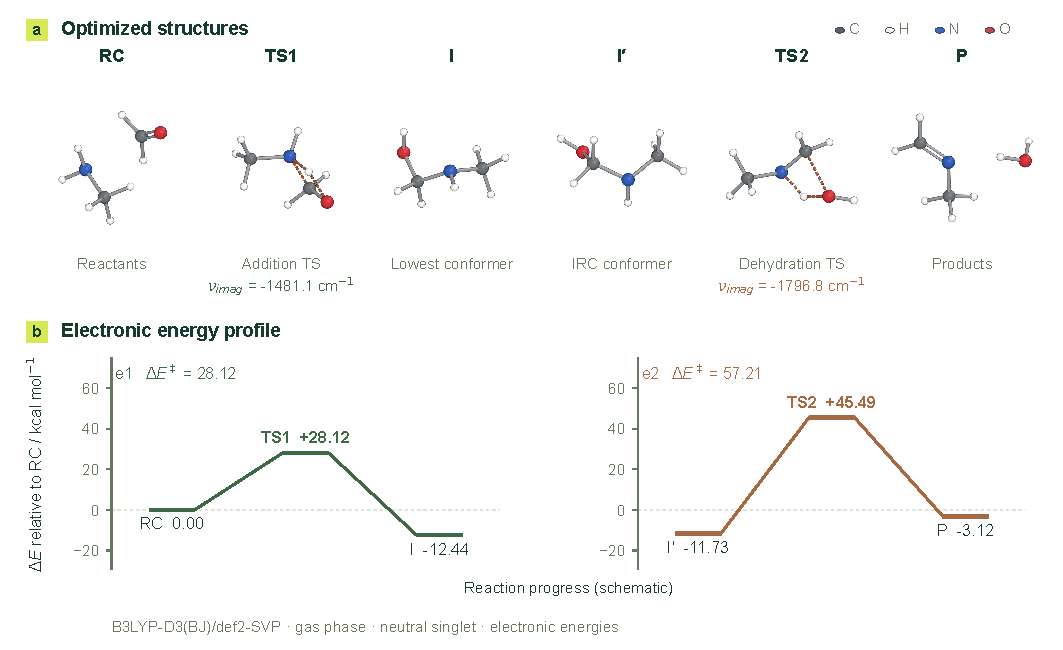
\includegraphics[width=\textwidth]{figures/fig_ni1_chemical_objects.pdf}
\caption{Two requested steps in the archived Guided/NI1 study: methylamine addition to formaldehyde and carbinolamine dehydration. Structures and electronic energies come from this run's B3LYP-D3(BJ)/def2-SVP gas-phase calculations. Each saddle has one imaginary frequency, and its short IRC branches lead through endpoint optimization/frequency analysis to minima with zero imaginary frequencies. The lowest carbinolamine conformer $I$ and the second step's actual IRC-side conformer $I'$ differ by 0.71 kcal/mol; their interconversion remains an uncomputed path.}
\label{fig:ni1-chemical-objects}
\end{figure*}

\begin{figure*}[!tbp]
\begin{minipage}{\textwidth}
\centering
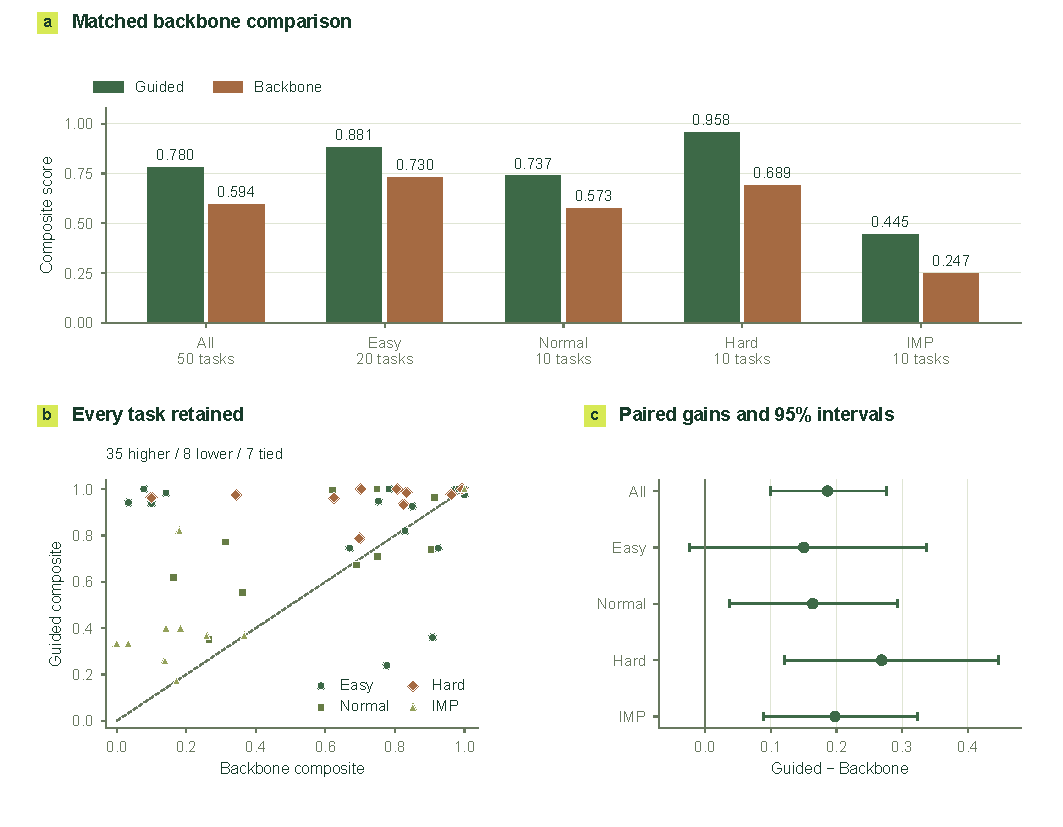
\includegraphics[width=\textwidth]{figures/bench_overview.pdf}
\caption{P2 benchmark outcomes under the archive-adjudicated track. (a) Guided and the same-backbone Standard baseline across all 50 tasks and each tier. (b) All 50 paired task outcomes. (c) Mean paired score differences with 95\% percentile intervals from 100,000 task-level bootstrap resamples. Each task has one run per configuration; Easy contains 20 tasks and the other tiers contain 10 each.}
\label{fig:bench-overview}
\end{minipage}
\end{figure*}

\begin{figure*}[!tbp]
\begin{minipage}{\textwidth}
\centering
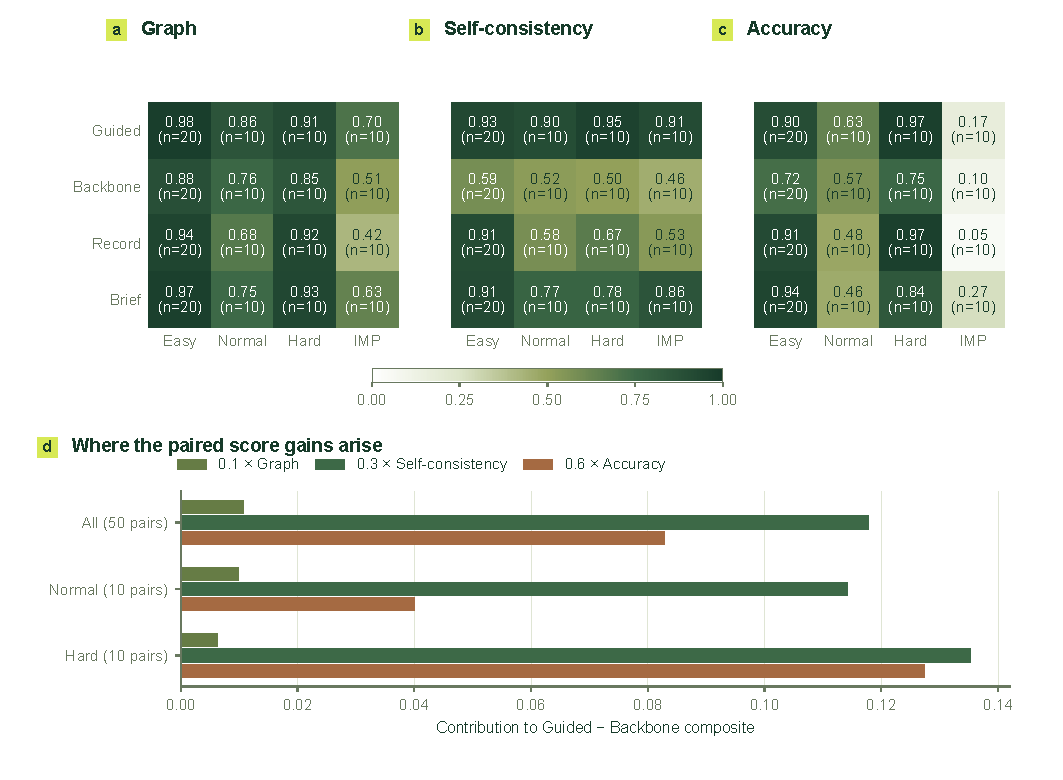
\includegraphics[width=\textwidth]{figures/bench_components.pdf}
\caption{CloudraBench score layers across all 200 organized runs. (a--c) Means of Graph, Self-consistency, and Accuracy in each arm and tier, using 50 tasks per arm overall, 20 Easy tasks, and ten tasks in each other tier. (d) Guided--Backbone mean differences decomposed with the fixed weights 0.1/0.3/0.6, using all 50 pairs, ten Normal pairs, and ten Hard pairs. The component values come from each run's final evaluation; their weighted sum gives the published composite score to the reported precision.}
\label{fig:bench-components}
\end{minipage}
\end{figure*}

\begin{figure*}[!tbp]
\begin{minipage}{\textwidth}
\centering
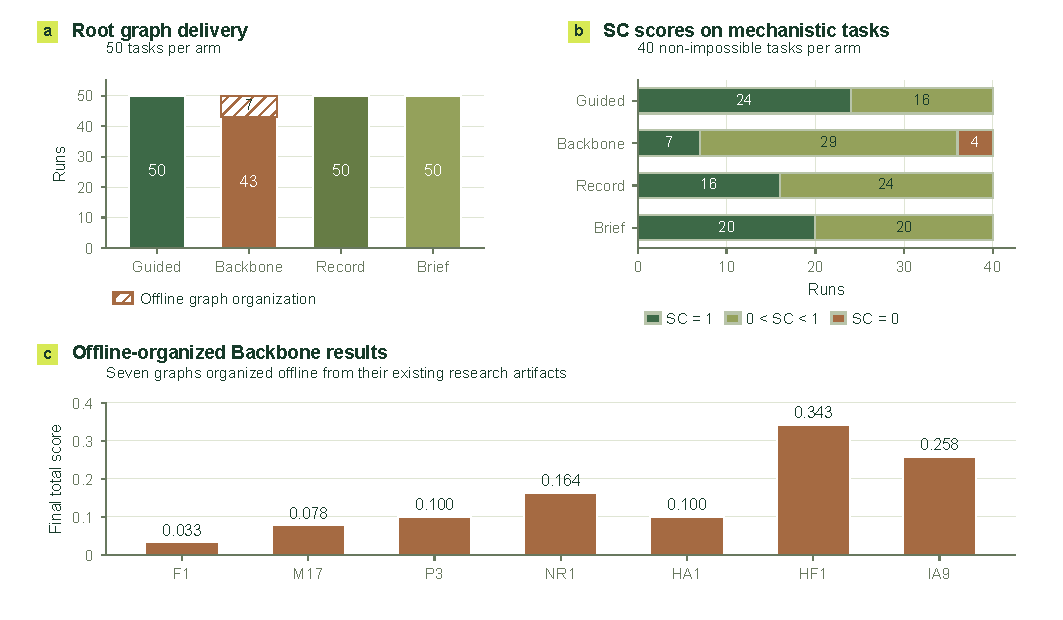
\includegraphics[width=\textwidth]{figures/bench_delivery.pdf}
\caption{Runtime graph delivery and final scientific support in P2. (a) Original root mechanism graphs across 50 tasks per arm: Guided 50, Backbone 43, Record 50, and Brief 50. The hatched segment marks seven additional Backbone graphs assembled offline from the runs' own research materials; the organized set contains 50 graphs per arm. (b) Final continuous self-consistency (SC) scores for all 40 non-Impossible tasks per arm, separating SC = 1, partial positive credit, and SC = 0. Full-score counts are 24, 7, 16, and 20; Backbone has four zero-score tasks. (c) Organized composite scores for the seven Backbone tasks whose root graphs were reconstructed offline, ranging from 0.0333 to 0.3425 (mean 0.1537).}
\label{fig:bench-delivery}
\end{minipage}
\end{figure*}

\begin{figure*}[!tbp]
\begin{minipage}{\textwidth}
\centering
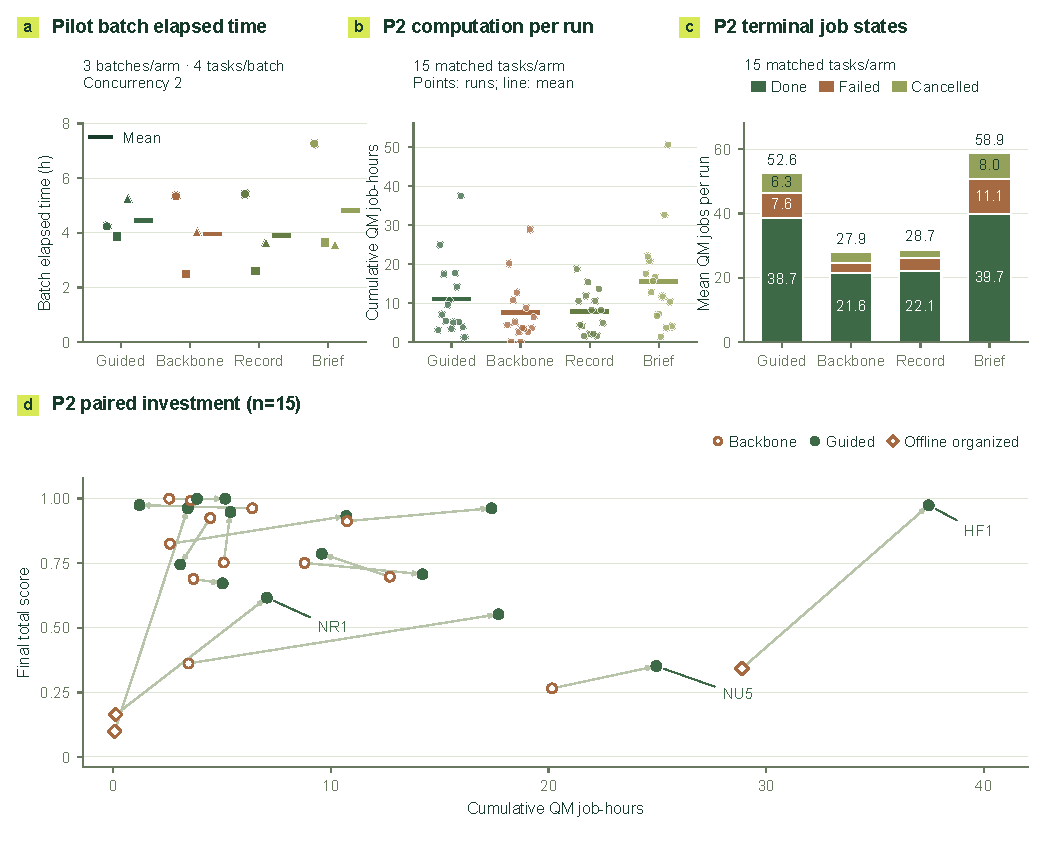
\includegraphics[width=\textwidth]{figures/bench_speed.pdf}
\caption{Research elapsed time and computational investment. (a) Twelve P1b four-task batches at concurrency two, three per arm; lines mark means. (b) Cumulative QM process durations for the 15 P2 tasks shared by all arms. (c) Mean completed, failed, and cancelled jobs in that cohort. (d) Same-task Backbone-to-Guided changes in investment and final score; diamonds mark offline-organized Backbone graphs. Job-hours sum process walltime; panel a measures batch latency. Backbone/M1 effort is reconstructed from native CPU time divided by four.}
\label{fig:bench-speed}
\end{minipage}
\end{figure*}

\begin{figure*}[p]
\begin{minipage}{\textwidth}
\centering
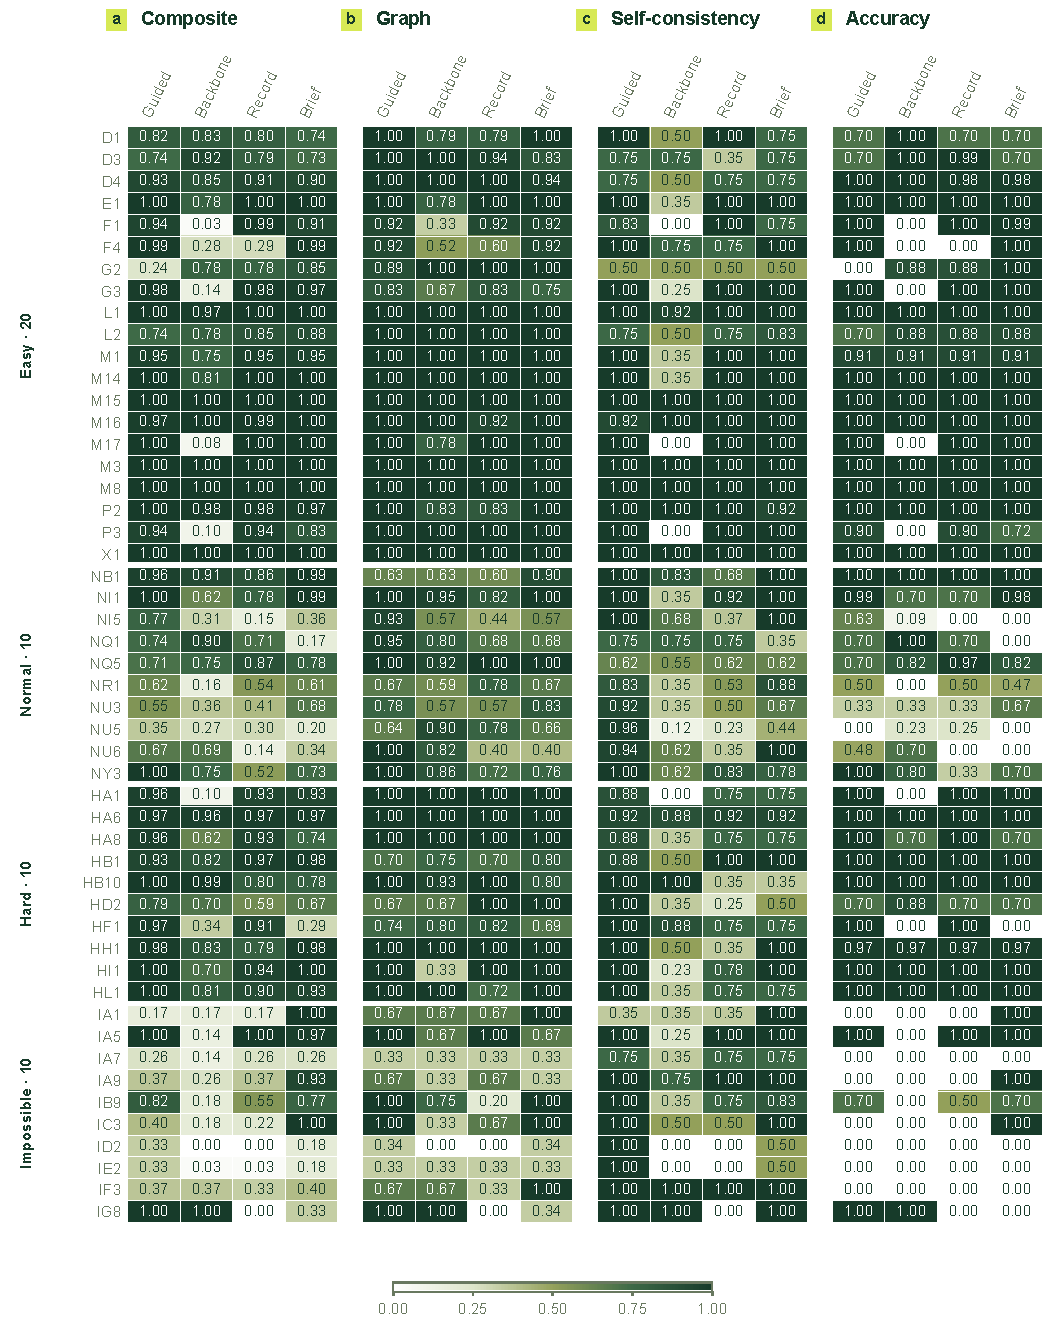
\includegraphics[width=\textwidth]{figures/bench_tasks_all.pdf}
\caption{Complete CloudraBench results for all 50 tasks and four configurations. The aligned blocks show composite, Graph, Self-consistency, and Accuracy on the same 0--1 scale; all 800 cells are present. Values are rounded to two decimals; the source table retains full precision.}
\label{fig:bench-tasks}
\vspace{6pt}
\end{minipage}
\end{figure*}

\begin{figure*}[!tbp]
\begin{minipage}{\textwidth}
\centering
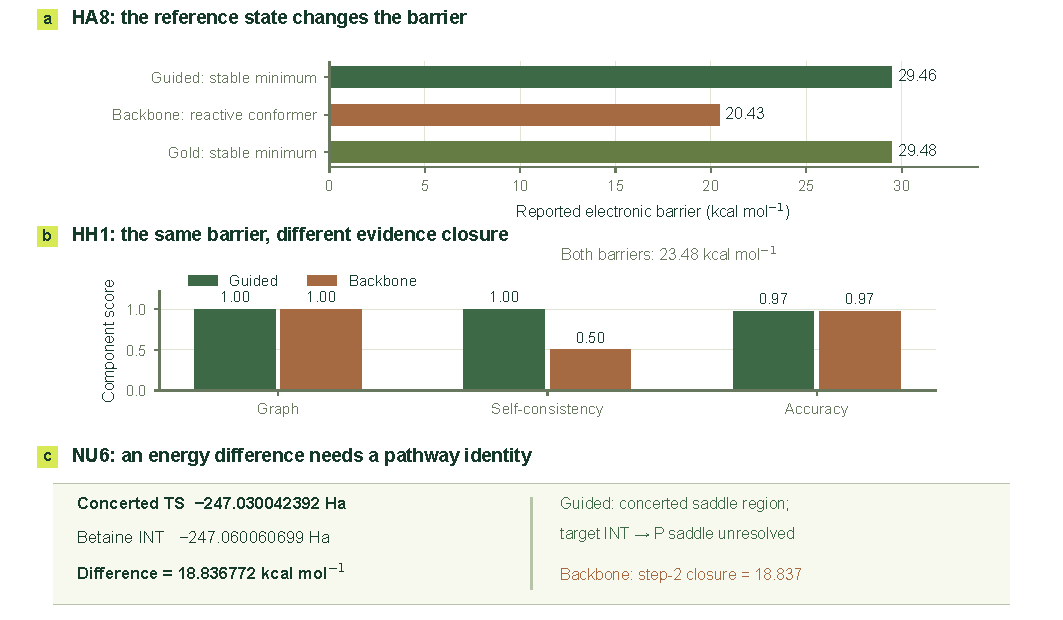
\includegraphics[width=\textwidth]{figures/bench_cases.pdf}
\caption{Energy references and pathway assignments in matched Guided--Backbone tasks. (a) HA8 barriers use a stable-minimum or reactive-conformer reference and are compared with campaign Gold. (b) Both HH1 runs report 23.48 kcal/mol with similar accuracy but different self-consistency scores. (c) NU6's recorded energy difference is 18.836772 kcal/mol: Guided reports the cost of reaching the concerted saddle region and leaves the target ring-closure saddle unresolved; Backbone reports 18.837 as the second-step ring-closure barrier. Values and assignments derive from the archived records.}
\label{fig:bench-cases}
\end{minipage}
\end{figure*}

\begin{figure*}[!tbp]
\begin{minipage}{\textwidth}
\centering
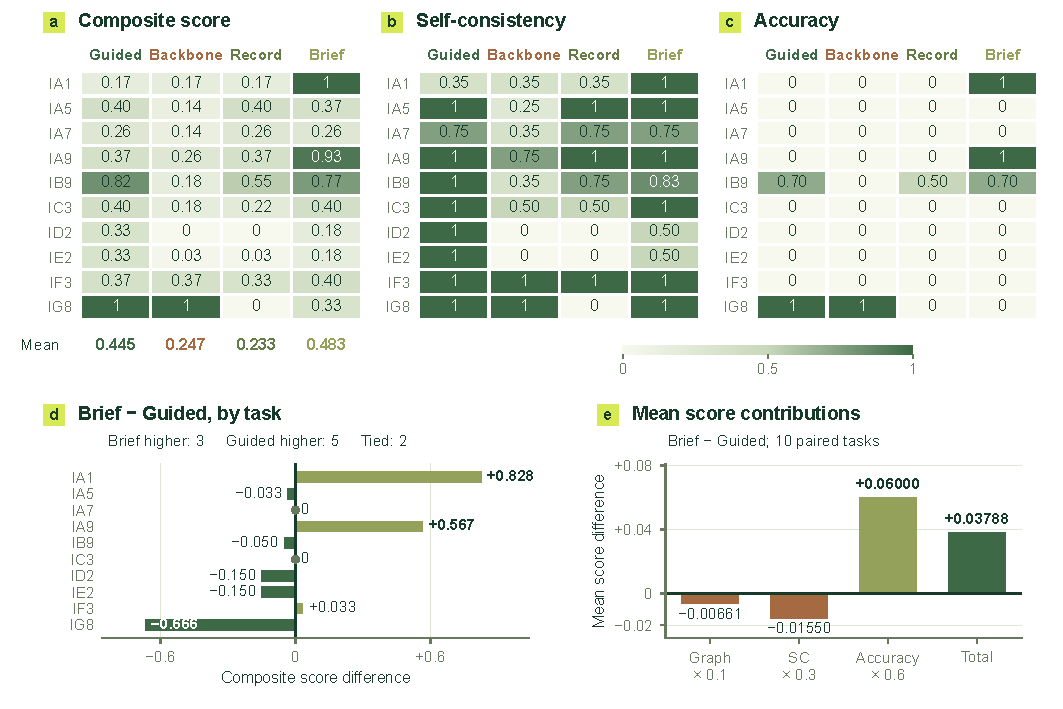
\includegraphics[width=\textwidth]{figures/bench_imp.pdf}
\caption{Impossible-tier outcomes after offline organization and scoring. (a--c) Composite score, self-consistency (SC), and accuracy for ten tasks and four arms, using the same complete scoring track and a shared 0--1 color scale. Backbone denotes the actual same-backbone Standard arm. Brief averages 0.603 and Guided 0.505. (d) Guided scores higher on 5 tasks, Brief on 4, and 1 tie. (e) The +0.09788 mean difference comprises accuracy +0.12000, Graph $-0.00661$, and SC $-0.01550$ after weighting; the small sum discrepancy reflects saved-score rounding. The paired task-bootstrap 95\% interval is $-0.160$ to $+0.361$. Accuracy zero does not universally indicate an incorrect refusal, and component or composite scores are not scientific acceptance rates.}
\label{fig:bench-imp}
\end{minipage}
\end{figure*}

\begin{figure*}[!tbp]
\begin{minipage}{\textwidth}

\centering
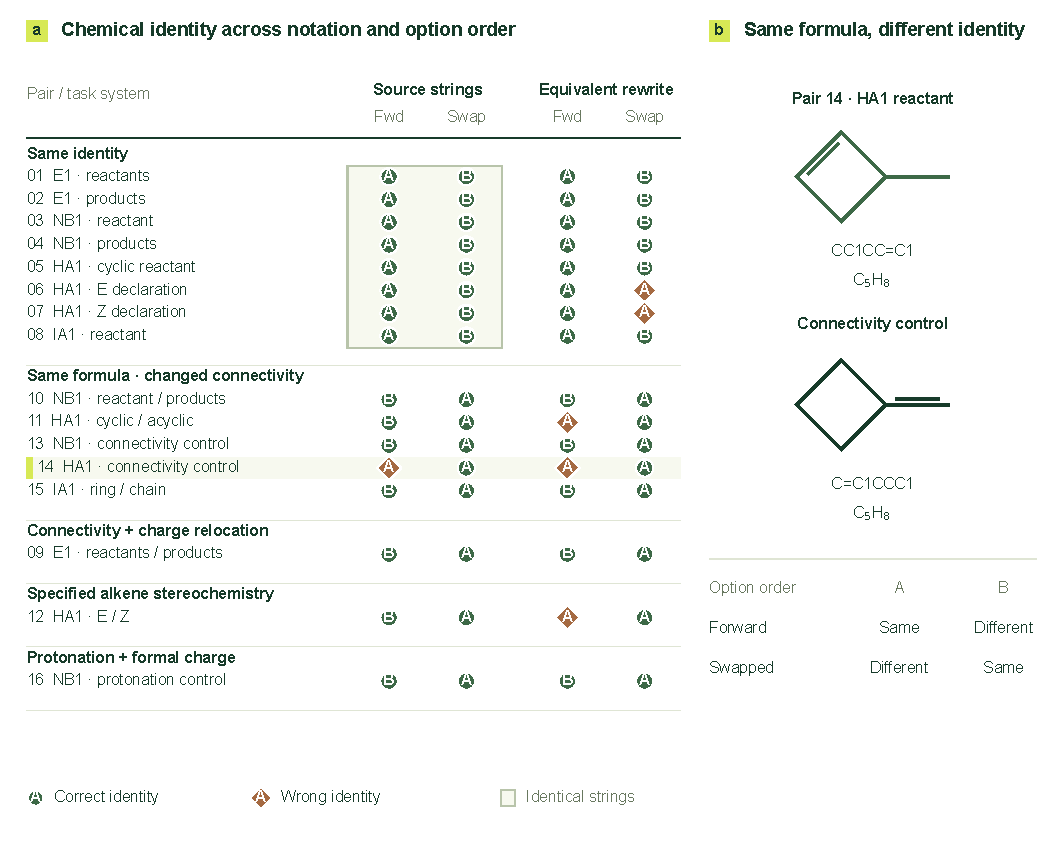
\includegraphics[width=\textwidth]{figures/fig06.pdf}
\caption{Molecular-identity judgments under changes in molecular representation and option order. Each of the 16 molecular pairs has four input conditions. Circles and diamonds indicate correct and incorrect judgments, respectively; the letters retain the model's actual answers. Shaded regions denote identical-string conditions. The right panel shows the pair-14 connectivities \texttt{CC1CC=C1} and \texttt{C=C1CCC1}, both C\textsubscript{5}H\textsubscript{8}, and the meanings of the answer options.}
\label{fig:06}
\end{minipage}
\end{figure*}

\begin{figure*}[!tbp]
\begin{minipage}{\textwidth}
\begin{minipage}[t]{.65\textwidth}
\vspace{0pt}
\centering
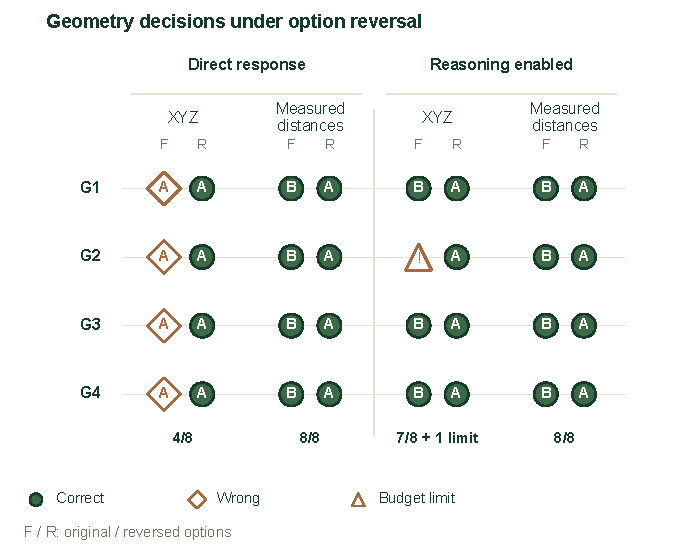
\includegraphics[width=\linewidth]{figures/fig07.pdf}
\caption{Judgments of which of two specified atom-pair distances is shorter, using coordinates or measured distances. Four source structures are compared under direct response and reasoning-enabled conditions, each with original (F) and reversed (R) option order. Circles indicate correct judgments, diamonds incorrect judgments, and the triangle a response that reached the output budget. Letters retain the actual answers.}
\label{fig:07}
\end{minipage}\hfill
\begin{minipage}[t]{.31\textwidth}
\vspace{0pt}
\centering
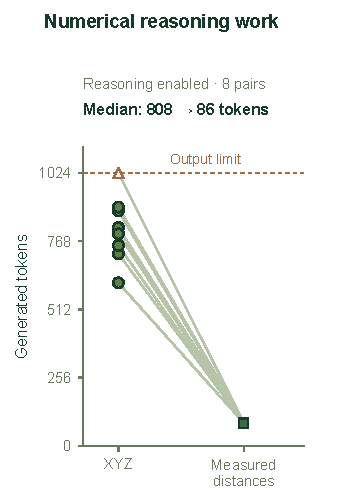
\includegraphics[width=\linewidth]{figures/fig08.pdf}
\caption{Generated-token counts with reasoning enabled. Each line connects Cartesian-coordinate input and measured-distance input for the same source structure and option order; eight paired comparisons are shown. The dashed line marks the output limit.}
\label{fig:08}
\end{minipage}
\end{minipage}
\end{figure*}

\begin{figure*}[!tbp]
\begin{minipage}{\textwidth}
\centering
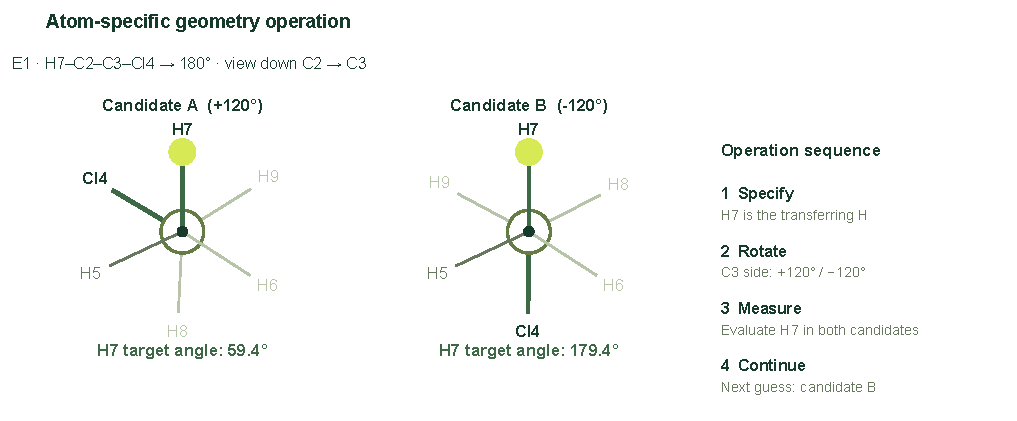
\includegraphics[width=.92\textwidth]{figures/fig09.pdf}
\caption{Target-specific geometry operations in E1. Newman projections retain the directions of the original candidate coordinates viewed down C2\(\to\)C3. H7 is the specified transferring atom. Candidate A and candidate B give target angles of 59.4° and 179.4°, respectively. The operation sequence is shown alongside the projections.}
\label{fig:09}
\vspace{5pt}
\begin{minipage}[t]{.48\textwidth}
\vspace{0pt}
\centering
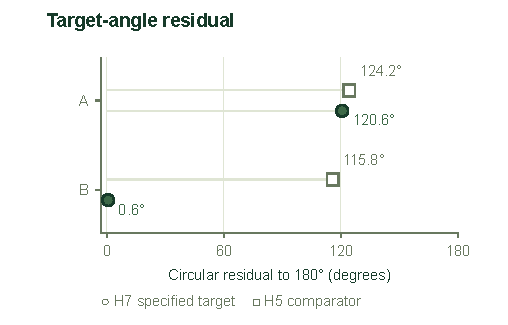
\includegraphics[width=\linewidth]{figures/fig10.pdf}
\caption{Circular angular residuals from the specified 180° target for candidates A and B. H7 is the specified target atom; H5 is the comparator.}
\label{fig:10}
\end{minipage}\hfill
\begin{minipage}[t]{.48\textwidth}
\vspace{0pt}
\centering
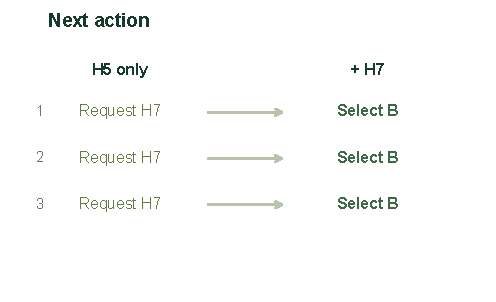
\includegraphics[width=\linewidth]{figures/fig11.pdf}
\caption{Next-action choices under three local option permutations. When only H5 measurements are supplied, the model requests H7 measurements; with H7 supplied, it selects candidate B.}
\label{fig:11}
\end{minipage}
\end{minipage}
\end{figure*}

\begin{figure*}[!tbp]
\begin{minipage}{\textwidth}
\centering
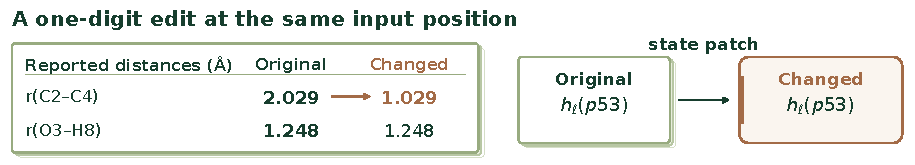
\includegraphics[width=.92\textwidth]{figures/fig12.pdf}
\caption{Intervention on a single reported distance. A one-digit edit changes the C2–C4 distance from 2.029 to 1.029 Å while O3–H8 remains 1.248 Å. The original-input residual state at token position 53 is inserted into the changed-input run at a specified layer. Token positions are zero-based.}
\label{fig:12}
\vspace{4pt}
\centering
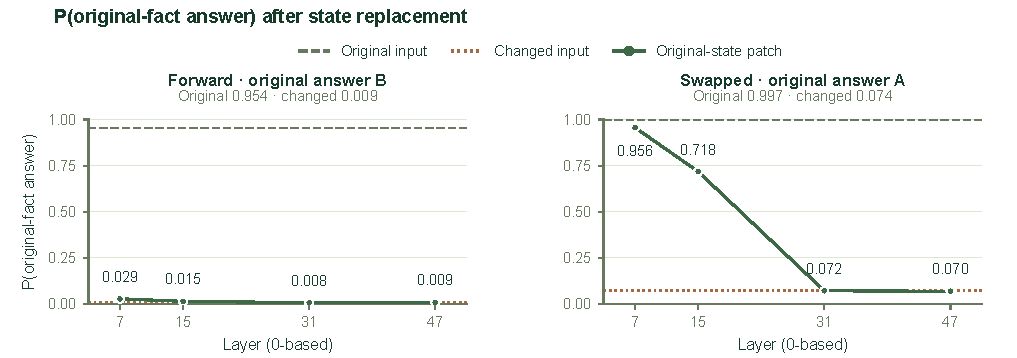
\includegraphics[width=.92\textwidth]{figures/fig13.pdf}
\caption{Original-fact answer probability after state replacement. Curves show full-vocabulary probability mass for the original-fact answer under forward (B) and swapped (A) option order, including bare and leading-space token spellings. Horizontal lines show original-input and changed-input baselines. Layer indices are zero-based.}
\label{fig:13}
\vspace{4pt}
\centering

\includegraphics[width=.92\textwidth]{figures/fig14.pdf}
\caption{Control substitutions for the state-intervention experiment. Same-state self replacement at p53 and replacement of the unchanged prefix at p0 preserve all vocabulary logits in both option orders. The table reports the maximum absolute logit difference. Token positions are zero-based.}
\label{fig:14}
\end{minipage}
\end{figure*}

\begin{figure*}[!tbp]
\begin{minipage}{\textwidth}

\begin{minipage}[t]{.48\textwidth}
\vspace{0pt}
\centering
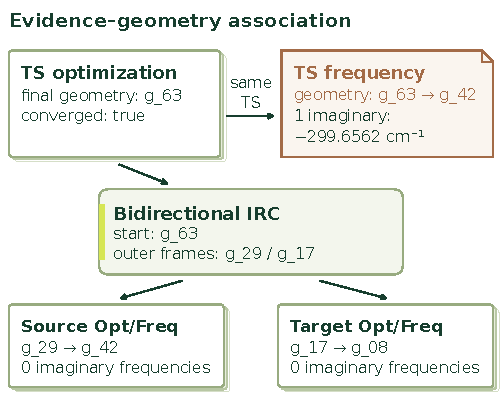
\includegraphics[width=\linewidth]{figures/fig15.pdf}
\caption{Changing the geometry assigned to the E1 frequency calculation. The frequency geometry reference changes from g\_63 to g\_42 while local termination, convergence, energy, and frequency values remain fixed. Arrows connect the TS, IRC, and endpoint optimization/frequency calculations.}
\label{fig:15}
\end{minipage}\hfill
\begin{minipage}[t]{.48\textwidth}
\vspace{0pt}
\centering
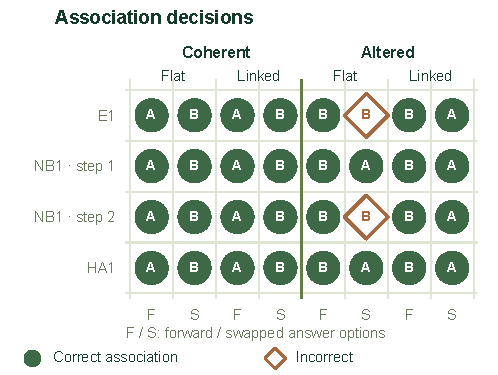
\includegraphics[width=\linewidth]{figures/fig16.pdf}
\caption{Judgments of whether calculation references support the specified step. The 32 inputs cross four source chains, coherent/altered links, flat/linked presentation, and forward/swapped answer order. Saved A/B responses and correctness markers are retained.}
\label{fig:16}
\end{minipage}
\end{minipage}
\end{figure*}

\begin{figure*}[!tbp]
\begin{minipage}{\textwidth}
\centering
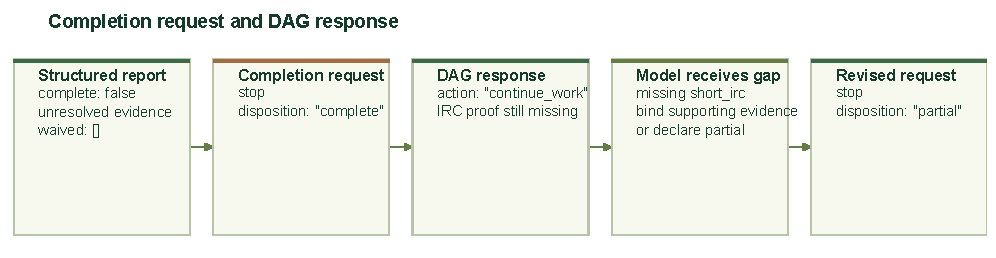
\includegraphics[width=.96\textwidth]{figures/fig17.pdf}
\caption{Completion requests and DAG feedback in the original IA1 trajectory. A report with unresolved evidence is followed by a completion request, a response identifying missing short\_irc proof, feedback to the model, and a revised partial-completion request.}
\label{fig:17}
\end{minipage}
\end{figure*}

\subsection{A two-step mechanism expressed through chemical objects}
\label{sec:ni1-chemical-objects}

The Guided NI1 run computes methylamine addition to formaldehyde and carbinolamine dehydration to an imine--water complex (Figure~\ref{fig:ni1-chemical-objects}). Its Delivery DAG connects the optimized reactant complex, carbinolamine, and product complex through two first-order saddles. Calculations used B3LYP-D3(BJ)/def2-SVP in the gas phase, with charge zero and singlet multiplicity.

The addition saddle has one imaginary frequency at $-1481.06$ cm$^{-1}$ and an electronic barrier of 28.12 kcal/mol relative to the reactant complex. Its two short IRC branches lead, after endpoint optimization and frequency analysis, to the reactant complex and carbinolamine, both with zero imaginary frequencies. The dehydration saddle has one imaginary frequency at $-1796.84$ cm$^{-1}$ and an electronic barrier of 57.21 kcal/mol relative to its IRC-side carbinolamine minimum. Its two branches similarly yield carbinolamine and the imine--water complex. Each IRC followed 24 points in each direction before reaching the point limit; the endpoint calculations establish the resulting minima.

Interconversion between the carbinolamine conformers remains uncomputed. Supplementary Information Section~S4 provides the conformer references, absolute energies, native calculation records, and figure inputs.





















\subsection{End-to-end benchmark evaluation}

CloudraBench measures end-to-end mechanism-calculation capability: constructing candidate mechanisms, carrying out the required quantum-chemical calculations, and reaching task-consistent positive or negative conclusions. We report composite scores together with their graph, self-consistency, and accuracy components. Offline postprocessing reconstructs mechanism graphs from each run's own research materials and compares the computed species, reaction channels, electronic states, and barrier references with the task definition. Before calculating Accuracy, we match each reported reaction channel and electronic state to the target specified in the task. All four workflows use the same postprocessing rules. The resulting 200-run table contains all three components for every run, with an overall composite mean of 0.7176. Figures~\ref{fig:bench-overview}--\ref{fig:bench-tasks} report runtime graph production, TS--IRC--endpoint evidence, and agreement with the task's answer.

\subsubsection{Cloudra improves end-to-end mechanism-calculation scores with the same backbone}

Guided obtained a mean composite score of 0.8050, compared with 0.5836 for Standard. Across the 50 task pairs, the mean improvement was 0.2214, with a 95\% task-bootstrap interval of [0.1349, 0.3124]. Guided scored higher on 35 tasks, lower on eight, and equally on seven; the median paired difference was 0.1142 (Figure~\ref{fig:bench-overview}).



Guided's mean over its ten lowest-scoring tasks was 0.3374, compared with 0.0930 for Standard.



The most consistent difference occurred in the Hard stereochemistry tasks. Guided averaged 0.9577 and Standard 0.6888, a paired increase of 0.2689 [0.1213, 0.4459], with Guided scoring higher on all ten tasks. These tasks require assigning each barrier and computed pathway to the corresponding stereoisomer or competing channel.

On Normal tasks, Guided averaged 0.7370 versus 0.5731, an increase of 0.1640 [0.0365, 0.2922], with seven wins and three losses. Easy-task means were 0.9125 and 0.7044, respectively; the paired median difference was 0.0209, showing a different pattern from the broadly positive Hard comparison. Impossible-task means were 0.5051 and 0.2473. Their interpretation depends on whether the run addressed the requested method-limited negative target, so these tasks are examined separately below.





\subsubsection{Self-consistency contributes most to the composite-score gain}

The three components score different parts of the calculation (Figure~\ref{fig:bench-components}). Graph measures the delivered coverage and identities of the requested species and steps. Self-consistency measures the support linking saddle points, frequencies, IRC starts, and endpoint optimization/frequency calculations. Accuracy measures agreement with the task's numerical or negative target. A run can therefore give a close numerical answer while leaving its supporting path incomplete, or establish a coherent local calculation that answers a different research question.

Across all 50 Guided--Standard task pairs, the weighted graph contribution to the mean improvement was +0.0108, self-consistency contributed +0.1179, and accuracy +0.0927, accounting together for the composite gain of 0.2214. For the 20 Normal and Hard tasks, the mean gain was 0.2164, with contributions of +0.0080 from graph, +0.1247 from self-consistency, and +0.0837 from accuracy. Within the ten Normal tasks, the corresponding contributions were +0.0098, +0.1141, and +0.0400; within the ten Hard tasks they were +0.0063, +0.1353, and +0.1274.



On Hard tasks, the weighted accuracy improvement is comparable in size to the self-consistency improvement.



HH1 provides a direct example. Guided and Standard both reported a binaphthyl racemization barrier of 23.48 kcal/mol, close to the 23.01 kcal/mol reference. Both had graph scores of 1 and accuracy scores of approximately 0.973. Their self-consistency scores were 1.0 and 0.5, producing composite scores of 0.9838 and 0.8338, respectively. The archived Standard study contained candidate channels and IRC inputs; the required endpoint connections remained unverified. Guided attached the path evidence to the corresponding saddle and endpoints. HI1 shows a related pattern: accuracy was approximately 1 in both runs, while self-consistency increased from 0.2333 to 1.0 and the composite score from 0.7032 to 0.9999. Establishing which minima the saddle connected therefore required the additional IRC and endpoint calculations.





\subsubsection{Delivery artifacts and graded scientific support remain distinct}

Runtime root-graph production is recorded separately from the physical evidence found in each run (Figure~\ref{fig:bench-delivery}). During the original runs, Standard delivered root graphs for 43 of 50 tasks, while Guided, Record, and Brief-errors each delivered 50. The seven Standard tasks requiring offline root-graph reconstruction were F1, HA1, HF1, IA9, M17, NR1, and P3. Offline organization assembled their graphs from the corresponding runs' existing materials, producing a complete 50-task set for every configuration. Recovering these seven Standard records credits research already performed by the baseline, making the comparison more conservative than withholding credit solely because the root delivery file was missing.

The seven Standard studies averaged 0.1537 after organization, compared with 0.8285 for Guided on the same tasks, and contributed 42.7\% of the total Guided--Standard difference. Their individual scores ranged from 0.0333 to 0.3425. Calculations and candidate descriptions could remain in a run's records while the requested pathway or comparative conclusion was unfinished. Offline organization recovers that existing content for evaluation.



For the 40 non-Impossible tasks in each configuration, Guided had self-consistency exactly equal to 1 on 24 tasks (60.0\%) and partial positive credit on 16. Standard had seven full-score (17.5\%), 29 partial-score, and four zero-score tasks. Record had 16 full-score (40.0\%) and 24 partial-score tasks; Brief-errors had 20 full-score (50.0\%) and 20 partial-score tasks. Figure~\ref{fig:bench-delivery} presents these complete evidence-score distributions alongside the separate runtime graph-delivery counts.

These percentages describe full self-consistency scores for the delivered objects. A task-wide scientific completion rate additionally requires physical support for every requested species and step. The archived runtime indicators cover delivered or agent-selected objects; a uniform check against all requested objects remains pending. Supplementary Information Section~S4 documents the scope of these records.

\subsubsection{Guided outperforms Record with the same available tools}

Record averaged 0.7038 and Brief-errors 0.7781 across all 50 tasks. Guided exceeded Record by 0.1012 [0.0396, 0.1695], with 28 wins, seven losses, and 15 ties. On all 20 Normal and Hard tasks together, the mean Guided--Record difference was 0.1468: graph contributed +0.0083, self-consistency +0.0919, and accuracy +0.0466. The largest contribution came from self-consistency, which scores the frequency, IRC, and endpoint calculations supporting the reported steps.





\subsubsection{Research batch times and quantum-chemical job-hours}

Figure~\ref{fig:bench-speed} presents the timing information from the repeated-task study alongside the computational effort available for P2. For the repeated study, the measurement unit is a complete four-task batch at a concurrency of two, with three observed batches per configuration. Mean batch elapsed times were 4.451, 3.958, 3.894, and 4.827 hours for Guided, Standard, Record, and Brief-errors, respectively. Guided batches took 12.5\% longer than Standard and 7.8\% less time than Brief-errors on average. The figure shows all 12 observed batches, retaining their variation and original outcomes. These measurements include the batch's research lifecycle, waiting for calculations, and continuation after results return.

P2 effort is summarized over the 15 deeply inspected tasks shared by all four configurations. Guided used 11.08 job-hours per task, Standard 7.55, Record 7.88, and Brief-errors 15.59. The corresponding final composite means were 0.8124, 0.6495, 0.7360, and 0.7273. Guided used 46.7\% more cumulative job time than Standard while increasing the mean score by 0.1629; relative to Brief-errors, it used 28.9\% less job time and scored 0.0851 higher. Guided was both faster in cumulative job time and higher-scoring than Brief-errors on seven of the 15 paired tasks.







Across the common tasks, Guided submitted 789 recorded quantum-chemical jobs, Standard 419, Record 431, and Brief-errors 883. Recorded failed-job counts were 114, 45, 62, and 167, respectively, with cancellations recorded separately. The four difficult studies NU3, NU5, NU6, and NR1 accounted for 163.5 job-hours across their 16 runs, 24.3\% of the 673.82 job-hours in the available 63-run effort archive. Some required steps in these four studies remained unresolved after additional attempts. In the archived Standard missing-graph cases, calculations could also outlive the research session, leaving subsequent results outside an active study.

Guided exceeded Brief-errors by 0.0268 overall, with an interval of [$-0.0486$, 0.0996], 26 wins, eleven losses, and 13 ties. The comparison varied by research demand: Guided's mean advantage was 0.1514 on Normal and 0.1295 on Hard, whereas Brief-errors had the higher Impossible mean.









\subsubsection{Uncapped electronic-barrier errors in a common numerical subset}

To express numerical deviations in chemical units, we recovered electronic barriers directly from archived native TS and reactant-reference energies. A common subset contains 26 reference edges from 23 positive tasks with recoverable values in all four configurations and components matching the final publication records. Edge assignments follow the task's specified reaction and energy-reference definitions. Table~\ref{tab:uncapped-barrier-errors} reports errors against the frozen task reference values, using each edge once per configuration and applying the energy conversion in Section~2.

\begin{table}[tbp]
\centering\small
\caption{Uncapped electronic-barrier errors for the same 26 reference edges in all four configurations, in kcal/mol.}
\label{tab:uncapped-barrier-errors}
\begin{tabular}{lrrr}
\toprule
Workflow & MAE & RMSE & Median $|\Delta|$ \\
\midrule
Guided & 1.17 & 2.86 & 0.057 \\
Standard & 1.54 & 4.64 & 0.057 \\
Record & 1.58 & 5.71 & 0.073 \\
Brief-errors & 1.13 & 2.31 & 0.099 \\
\bottomrule
\end{tabular}
\end{table}

These errors retain large deviations that the composite Accuracy component's penalty cap compresses. Guided has a lower MAE and RMSE than Standard in this subset, while Brief-errors has the lowest MAE and RMSE. The subset describes recoverable numerical answers; frequency and pathway support are evaluated separately by self-consistency. SI Section~S4 gives every included value, the coverage of the 53 positive numerical reference edges, and a smaller subset with additional Gold-input method and medium corroboration. The numerical ordering varies with that coverage.

\subsubsection{Per-task comparisons of barriers, pathways, and calculation evidence}

Figure~\ref{fig:bench-tasks} places all 50 tasks and four configurations alongside their complete score components. NB1 and NI1 also illustrate the scores obtained on multistep mechanisms. NB1 scored 0.9628 under Guided, 0.9128 under Standard, and 0.9900 under Brief-errors; Guided and Brief-errors both had self-consistency 1. NI1 scored 0.9958 under Guided and 0.6196 under Standard, with self-consistency 1 and 0.35. In contrast, NQ5 favored Record over Guided, and NU3 favored Brief-errors.

The archived records explain several barrier differences (Figure~\ref{fig:bench-cases}). In HA8, Guided reported 29.46 kcal/mol and Standard 20.43 kcal/mol against a reference of 29.48 kcal/mol. The archive traces this 9.03 kcal/mol difference to the energy reference: the lowest all-s-trans reactant minimum in Guided and a reactive cisoid conformer in Standard. The IRC identifies the local structures connected by the saddle; the reported activation energy uses the stable-minimum reference specified by the task.



NU6 exposes a related issue in path identity. Guided's recorded concerted saddle had an energy of $-247.030042392$ Ha and the betaine minimum $-247.060060699$ Ha, giving a difference of 18.836772 kcal/mol. Guided described this as an energy cost involving the concerted saddle region while retaining the target betaine-to-product ring-closure saddle as unresolved. Standard delivered 18.837 kcal/mol as the second-step ring-closure barrier. The two reports assign this nearly identical energy difference to different processes. Guided's attempts from interpolated betaine structures and constrained scan peaks repeatedly relaxed toward the direct reactant-to-product saddle region. The saddle's path identity therefore required another assessment from its optimized geometry and pathway.



In G2, Guided scored 0.2389 and Standard 0.7769. Guided's native logs supported an approximately 0.845-kcal/mol double-H-transfer barrier. After three rejections of numerical barrier declarations on a companion edge, the agent removed the numerical fields. Supervisor feedback prompted restoration; a fourth rejection and a subsequent saddle-evidence check preceded their final removal, together with the saddle energy/log bindings. The final graph retained the values in text and received accuracy 0. Brief-errors retained the corresponding numerical result and scored 0.8500.

The accuracy values of 0.7 in D1 and D3 followed the specified cap on numerical-deviation penalties. D1's barrier difference from Standard traced to the reactant-conformer reference; D3's mainly reflected different saddle energies. The Supplementary Information provides the workflow-level components and native calculations for these case studies.





\subsubsection{Impossible tasks distinguish local support from the requested negative conclusion}

The Impossible tier tests whether research identifies the requested target as physically inaccessible under the permitted xTB/PM7 methods. Offline postprocessing applies channel and electronic-state correspondence uniformly before Accuracy, so negative-target credit follows the pathway or state requested by the task. Brief-errors averaged 0.6029, Guided 0.5051, Standard 0.2473, and Record 0.2925 (Figure~\ref{fig:bench-imp}). Brief-errors exceeded Guided on four tasks and scored lower on five, with one tie. The Brief-errors-minus-Guided mean was +0.09788, with a 95\% task-bootstrap interval of [$-0.160$, $+0.361$]. Its weighted contributions were $-0.00661$ from graph, $-0.01550$ from self-consistency, and $+0.12000$ from accuracy. Task-level Brief-errors-minus-Guided differences were IA1 $+0.8283$, IA9 $+0.5666$, IC3 $+0.6000$, IF3 $+0.0333$, IA7 $0$, IA5 $-0.0333$, IB9 $-0.0500$, ID2 $-0.1500$, IE2 $-0.1500$, and IG8 $-0.6661$.

In IA1, concerning cyclobutadiene's square-geometry automerization target, Brief-errors had graph, self-consistency, and accuracy scores of 1, while Guided's accuracy was 0. In IA9, concerning dioxetane thermolysis, Brief-errors and Guided both had self-consistency 1, with accuracy 1 and 0, respectively. IG8 showed the opposite accuracy ordering for the chromium-dimer target. After target correspondence, Guided, Record, and Brief-errors received full negative-target Accuracy credit on IA5 (thermal disrotatory ring opening), and Brief-errors received full credit on IC3 (open-shell singlet phenylnitrene); Guided/IC3 retained Accuracy 0 with Graph and self-consistency both 1. Across the six tasks with the same accuracy score in Brief-errors and Guided, Brief-errors averaged 0.0583 lower. The higher Brief-errors mean therefore arose from the requested conclusions on specific tasks, while Guided retained stronger local support on several others.



Across all 40 Impossible runs, eight had accuracy 1 and ten combined self-consistency 1 with accuracy 0. IF3 illustrates the latter pattern: Brief-errors and Guided both had Accuracy 0 with self-consistency 1. Guided and Brief-errors both received partial accuracy of 0.7 in IB9, whose requested network contains positive and negative components.


















\subsection{Molecular identity, distance comparison, and fragment rotation}


We next examine whether the model distinguishes molecular identities, compares distances between specified atoms, detects mismatched calculation references, and identifies missing IRC calculations. Archived research trajectories supply the molecular structures and calculation records. Controlled local studies with Qwen3.8:27b vary the supplied information, answer order, and selected internal states to test their effects on each judgment.

\subsubsection{Equivalent SMILES and answer order affect molecular-identity judgments}
\label{sec:identity-judgments}



A geometric modification first requires identifying the molecule, atoms, and reaction center to which it applies. A molecule can be represented by different SMILES traversals, while a molecular formula can describe different connectivities. To examine how the model handles these distinctions, we constructed 16 molecular-identity pairs covering identical identities, connectivity changes within the same molecular formula, changes in connectivity and charge location, double-bond stereochemistry, and protonation changes. Each pair was presented using the original strings or equivalent rewritings and with two answer orders, yielding 64 judgments.



The model answered 58 correctly. Equivalent rewriting changed the semantic judgment in 4 of 32 matched representation comparisons; reversing answer order changed the judgment in 6 of 32 matched option-order comparisons. All six of the latter cases involved repeated selection of the letter A. One C\textsubscript{5}H\textsubscript{8} pair in Figure~\ref{fig:06} illustrates this behavior directly: an endocyclic and an exocyclic double bond define different connectivities, yet the model answered A under all four conditions, although A meant “same” in one order and “different” in the other. Thus, changing the notation or answer order can change whether the model judges two structures to be the same molecule.

Cloudra stores molecular connectivity separately from coordinates and uses atom correspondence to identify which atoms to measure, move, or compare. Product-endpoint alignment, path interpolation, and reaction-center measurements retain this correspondence as the structure's coordinates change.





\subsubsection{Geometric measurements reduce repeated numerical reasoning}

We selected four actual structures from the NB1 trajectories and asked the model which of two specified interatomic distances was shorter. Each structure was presented with both answer orders and with either a complete XYZ geometry or program-measured distances. These two information conditions were further crossed with direct-answer and thinking modes, producing 32 native chat calls (Figure~\ref{fig:07}).

In direct-answer mode, all eight responses to XYZ inputs selected A, with four correct answers. Providing measured distances produced eight correct answers and preserved the semantic answer when option order was reversed. With thinking enabled, the XYZ condition produced seven correct answers; the remaining response reached the output limit of 1,024 generated tokens. Increasing the budget for that input alone yielded a correct answer within 1,353 generated tokens. 

All eight answers in the measured-distance condition were correct. Across the eight paired comparisons with thinking enabled, the median generated token counts were 807.5 for XYZ inputs and 86 for measured distances.

Providing the distances removes the need for the model to calculate them from XYZ coordinates. Cloudra similarly computes bond lengths, bond angles, and dihedral angles in software and uses deterministic operators to rotate or translate the selected fragments. The model chooses the atoms and target geometry, then compares the measured distances or angles of the resulting candidates. Assigning these numerical operations to software follows the approach of program-aided language models.\citep{ref15}





\subsubsection{Feedback must match the specified atoms and geometric objective}



In an actual E1 trajectory, the model sought to bring the dihedral angle defined by the transferring hydrogen H7, C2, C3, and leaving atom Cl4 close to 180°. It rotated the fragment on the C3 side about the C2–C3 axis by +120° and \( - \)120°, producing candidates A and B, and set the C3–Cl4 distance to 2.35 Å. The representative dihedral in the default structure report involved H5, whereas the current objective involved H7. The model then explicitly measured H7–C2–C3–Cl4 in both candidates, obtaining approximately 59.4° and 179.4°, and used candidate B in its next actual submission.

Figure~\ref{fig:09} shows Newman projections along C2\(\to\)C3 drawn directly from the saved candidate coordinates, and Figure~\ref{fig:10} summarizes the corresponding target-angle residuals. Candidate B places the H7 target angle within 0.6° of 180°, compared with a residual of 120.6° for A. 

The corresponding residuals for the H5 comparison were 124.2° and 115.8° in A and B, respectively. Identifying the anti-periplanar H7--Cl4 arrangement in B required the H7-based dihedral.

When local probes provided only H5 measurements, the model requested an additional H7 measurement under all three cyclic option permutations. Adding H7 measurements led it to select B under all three permutations. Two further paired tests of information sufficiency also shifted from requesting additional measurements to judging the information sufficient when the target quantity was added.





\subsubsection{Activation replacement affects distance answers differently across option orders}

To test how a reported distance affects the answer, we performed activation replacement at a single token position in the same local quantized model.\citep{ref16} One distance in the input was changed from 2.029 Å to 1.029 Å, while the other remained at 1.248 Å, reversing the correct comparison answer. We then transferred the residual-stream state at the numeric token position from the original input into the modified input at layers 7, 15, 31, and 47, and read the full-vocabulary probability assigned to the answer supported by the original fact.

The effect varied with layer and option order (Figure~\ref{fig:13}). With reversed options, the probability of A, the original-fact answer, increased from 0.074 for the modified input to 0.956 and 0.718 after replacement at layers 7 and 15, respectively. Replacements at layers 31 and 47 yielded 0.072 and 0.070. With the original option order, the probability of answer B changed from 0.009 to 0.029 and 0.015 after replacement at the first two tested layers, while the last two remained close to the modified-input baseline. 

Self-replacement controls and control replacements at an unchanged prefix position produced zero logit differences across the full vocabulary.

With reversed options, replacing the early-layer state restored the original-fact answer as the preferred choice; with the original option order, the modified-fact answer remained preferred. Recovering the answer from the same numeric position therefore depended on option order, as did the identity judgments in Section~\ref{sec:identity-judgments}.


\subsection{Identifying the species and pathways established by calculations}


\subsubsection{Associating frequencies and IRC endpoints with the same saddle}

Once geometric objects enter computation, optimized structures, energies, frequencies, and paths must be assembled into support for the same reaction step. The local validity and attribution of each result jointly determine this support chain: frequencies must correspond to the declared saddle point, the IRC must start from that saddle point, and optimizations and frequencies for the final frames on both sides must correspond to the respective endpoints. The DAG attaches the optimized geometry, frequency calculation, IRC start, and endpoint calculations to the corresponding species or step. It records job execution, optimization convergence, and these physical checks separately; a converged optimization can still require frequency or endpoint calculations.

We extracted four source evidence chains from the archive and constructed versions that preserved the links or changed a single reference. Crossing these with flat and linked representations and two answer orders yielded 32 inputs. The altered references concerned the frequency geometry, IRC starting geometry, endpoint-optimization input, or target species; local termination, convergence, energy, and frequency values were held constant. Figure~\ref{fig:15} illustrates the E1 case: changing the frequency geometry reference from the saddle point to an existing endpoint changes how that frequency result supports the current step.

All 16 judgments with linked representations were correct, compared with 14 of 16 with flat representations. Both errors occurred when a reference had been changed and the options reversed, in E1 and the second NB1 step. In subsequent native follow-up calls on two selected source chains, enabling thinking yielded correct judgments for all 16 judgments of the evidence relationships, including the two previously incorrect cases. 

The model detected every altered reference in the linked format, even though the local numerical values were unchanged. This presentation effect is consistent with observations that graph encoding affects relational reasoning in language models.\citep{ref17} Cloudra records the corresponding artifact references for each species, step, and calculation attempt, identifying which saddle, IRC, and endpoint calculations are being compared.

\subsubsection{Diagnostic feedback on IRC connectivity and transition-state curvature}

Diagnostic feedback connects an evidence defect to the chemical object and calculation that require revision. Cloudra's structured diagnostics identify specific problems in quantum-chemical outputs, including steric-clash atom pairs, imaginary-mode misalignment, and disconnected trajectory endpoints. The agent can then change the clashing geometry, inspect the imaginary mode, or recalculate the affected endpoint.

Two archived trajectories illustrate this connection. In a Brief-errors HA1 trial, compact error codes replaced the detailed IRC-endpoint linkage diagnostics. The Computational Agent repeatedly substituted source-minimum references while the geometric disconnection remained unresolved. In a Guided NB1 trial, the verification found zero imaginary frequencies and returned a normal-mode diagnostic. The Coordinator requested a retry with revised transition-state guess parameters and optimization constraints, which the Computational Agent used in the rescheduled calculation.\citep{ref18}



\subsubsection{IA1: a completion request with a missing IRC calculation}

An archived IA1 trajectory shows how a completion request can conflict with the recorded scientific requirements. The reaction step had mandatory bidirectional short\_irc verification pending, and the waiver list was empty. The Supervisor had earlier commented positively on intermediate optimization convergence. The model subsequently requested completion while the IRC requirement remained unresolved.

The harness rejected that request and returned the outstanding short\_irc requirement to the model. In the next submission, the model changed its status to partial completion (Figure~\ref{fig:17}). The missing IRC calculation remained unresolved when the completion status changed.

We also tested whether the model could identify the outstanding IA1 requirements from the recorded state. All 12 judgments were correct (100\%) across six pairs with reversed answer-option order, using both a minimal summary and an extended 12-message history.

\subsection{Workflow guidance, scientific judgment, and outlook}

Across the 50-task comparison, Guided had higher mean self-consistency and accuracy than Standard. On Hard tasks, their weighted contributions to the gain were +0.1353 and +0.1274. The HH1 and HI1 results show how IRC and endpoint calculations establish the connections behind reference-consistent barriers.

HA8 and NU6 show why energy references and saddle assignments must follow the computed structures and paths. In HA8, the stable reactant minimum defines the barrier reference, while the IRC connects the saddle to a local reactive conformer. In NU6, guesses for betaine-to-product closure repeatedly optimized toward the direct reactant-to-product saddle region. The DAG keeps the reactant conformer, saddle, IRC endpoints and assigned step together so that the agent can check which structure each energy belongs to after a new calculation. The calculations provide external feedback for the agent's planning and verification.\citep{valmeekam2023planning}

These cases call for different next steps: calculate a missing endpoint, revise a guess that returns to another route, or reassess a method that cannot describe the requested electronic state. The agent must update its reaction description when the computed structures or paths change.\citep{turpin2023unfaithful} Record retained the tools and obtained lower self-consistency than Guided, particularly on Normal and Hard tasks. The archived trajectories show how tool feedback directs the next geometric operation or calculation.\citep{ref18,huang2024selfcorrect}

Brief-errors scored higher on IA1 and IA9, whereas Guided scored higher on IG8. These crossed outcomes motivate a task-dependent hypothesis: detailed diagnostics may help repair a TS or IRC calculation, with limited benefit from further local repair when the method or target needs reconsideration.

In G2, repeated checks led the agent to delete numerical values already supported by native calculations. Supervisor feedback restored the fields before further rejection led to their final deletion. A numerical observation and its log should remain attached to the graph while its mechanistic assignment is being tested.

P2 contains one run per task and configuration; its task-cluster bootstrap intervals describe variation across tasks. P1b provides three repeats on each of four tasks under each configuration, totalling 48 runs. Some Hard-task Accuracy targets score qualitative channel identity, so the reported gain includes pathway identification and evidence completion as well as numerical barriers.

Standard sometimes ended research while calculations were still running, whereas Guided/HI1 remained waiting after the completion notification. Returning results therefore need to resume the unfinished study before final reporting. NU6's repeated convergence to one saddle region also motivates comparing new candidates with previous attempts before choosing another guess.

Default preorganization samples 32 rigid relative placements and selects locally relaxed MMFF94 candidates by energy and clustering. CREST provides additional sampling through an optional backend.

The benchmark scores electronic energy differences, including the prescribed references for NI5 in weakly acidic aqueous solution and NU5 in concentrated dichloromethane. Solution-phase $\Delta G^\ddagger$ profiles would include zero-point, thermal/entropic, standard-state and solvation contributions. Solvent participation can also change the chemical model used to describe a pathway; solvent sensitivity remains to be assessed.

The workflow comparisons use fixed atom-mapping and branch-crowding settings and the DeepSeek-v4.1-flash (1017) backbone, with API alias \texttt{deepseek-v4-flash}.

Cloudra is publicly available as open-source software under the GNU Affero General Public License (AGPL) at \url{https://github.com/yyywaa/Cloudra-mechanism-agent}, supporting inspection, reuse, and community development of the system. Reproducible tables and scores are in the companion data package.

